

\subsection{Customer Requirements}
A fully functional semi-automatic annotation tool is expected. It should
provide flexible methods for easing the post inspection and correcting.
Besides, it should provide the following functionalities:

\subsubsection{Qualitative Requirements}
\begin{enumerate}
    \item \textcolor{gray}{A tidy user interface}
    \item \textcolor{gray}{Road object detection}
    \item \textcolor{gray}{Pedestrian pose estimation}
    \item \textcolor{gray}{Simplified tag list}
    \item \textcolor{gray}{Distinguishable tag category}
    \item \textcolor{gray}{High labeling speed}
    \item \textcolor{gray}{High Labeling coverage}
    \item \textcolor{gray}{Online deployment}
\end{enumerate}

\subsubsection{Specific Functional Requirements}
\begin{enumerate}
    \item \textcolor{gray}{Attributes such as occluded, truncated are included
in our labels. }
    \item \textcolor{gray}{Different traffic signs, lights, car lines can be
identified with our deep learning models.}
    \item \textcolor{gray}{Pedestrian are identified with their pose labeled.
These labels also include the attributes such as occluded, non-occluded,
not-in-picture, etc.}
    \item \textcolor{gray}{Some additional user-friendly features are
introduced:} \begin{itemize}
        \item \textcolor{gray}{Inverse-selection of the polygon region to be
labeled.}
        \item \textcolor{gray}{Move/Zoom-in the pictures}
        \item \textcolor{gray}{Match the labels in the pictures with the
polygons}
        \item \textcolor{gray}{Copy and paste between the pictures.}
        \item \textcolor{gray}{Color differentiation of different label types}
        \item \textcolor{gray}{Transparency of the irrelevant objects when
labeling a specific object. }
    \end{itemize}
    \item \textcolor{gray}{Data can be uploaded and the tool can be used online
for safer data transaction.}
    \item \textcolor{gray}{All the output are in a \texttt{.json} format,
specifying location, category, attributes, for better future training of deep
learning models.}

    \item The annotation tool is deployed online. Based on the automatic
generated preprocessing outcome, multiple users can do the manual correction at
the same time without conflict. Our work here is to port our GUI in the second
part to the web frontend and establish a backend database and computing logic
to perform the automated annotation.
\end{enumerate}


\subsection{Quality Function Deployment (QFD)}
\textcolor{gray}{Including all the customer requirements and engineering
requirements, we collect the information and create the QFD chart in Fig.
\ref{fig:qfd}. We consider high labeling speed and high labeling coverage as
the two most important customer requirements. Road object detection and
pedestrian pose estimation also play significant roles. The weight is graded
and 10 represents the highest demand while 1 represents a lowest one. We
transfer this information into the engineering requirements with quantified
terms, and list them on the top of the chart. In the middle part, we score the
correlation between customer requirements and engineering specifications. 9
represents a strong relationship, 3 represents a medium one and 1 means a small
relationship. If there is a blank, it means no relation exists between these
two.}

\textcolor{gray}{Then, we multiply the scores between corresponding quantified
and qualified requirements to obtain the total scores. The measurements units,
normalized scores and rank orders are also shown with the total scores at the
bottom of the chart. We place the competitive benchmark - Labelme at the right
of the chart and score it with the listed customer requirements. In addition to
these, the engineering specifications have potential correlation between
themselves. Therefore, we put the evaluation in the top triangle. The '+'
symbol shows a positive relation while '-' shows negative one. }
\begin{figure}[htbp]
  \centering 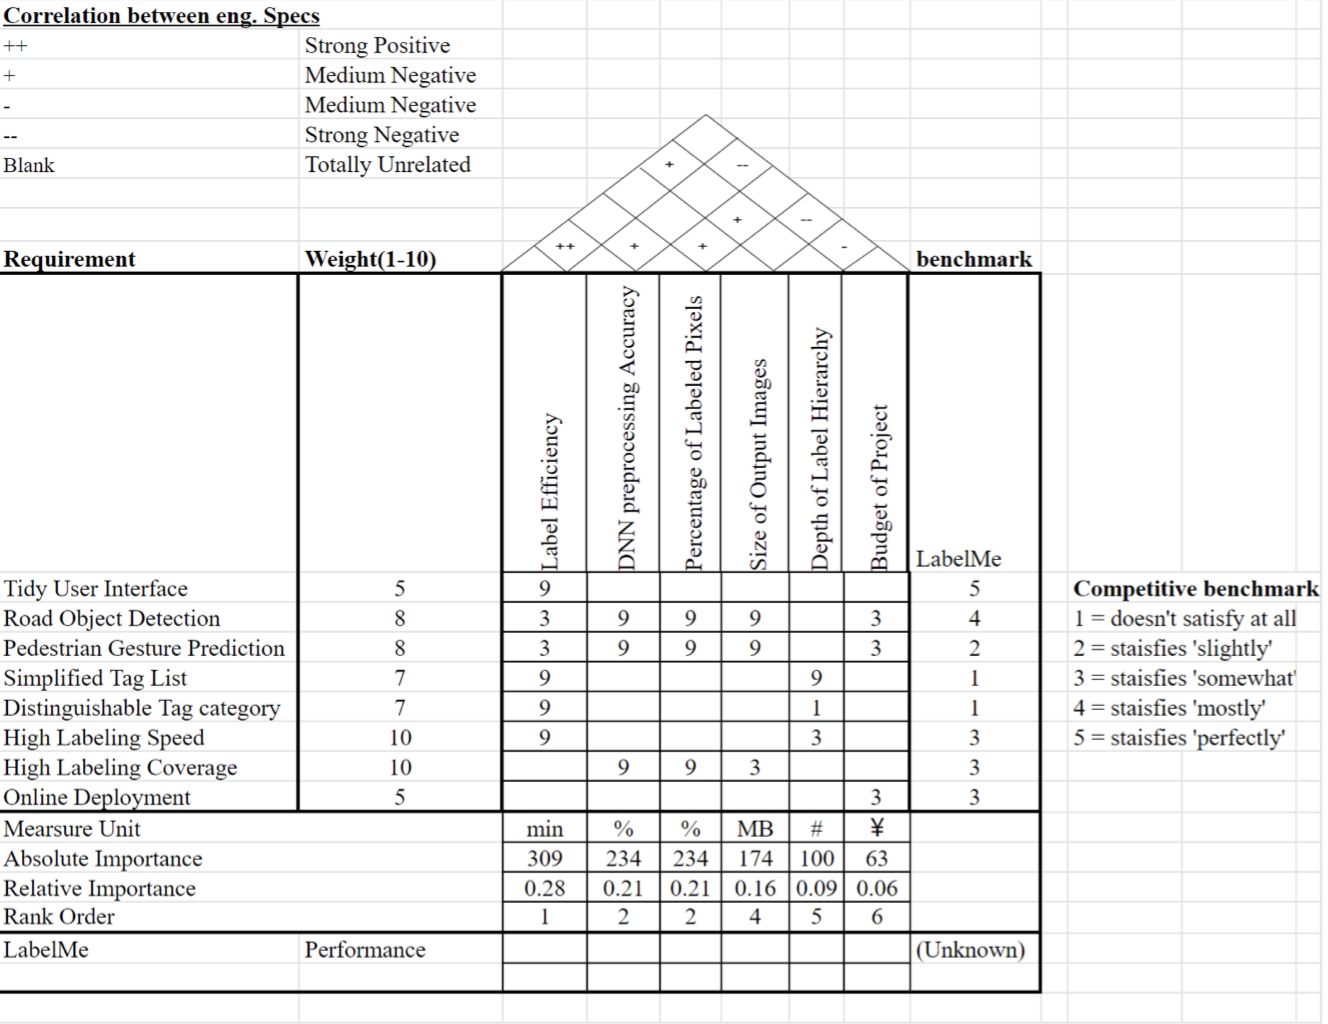
\includegraphics[width=\linewidth]{qfd2.png} % insert QFD here
  \caption{Quality Function Deployment}
  \label{fig:qfd}
\end{figure}
